\documentclass[%
reprint,
%superscriptaddress,
%groupedaddress,
%unsortedaddress,
%runinaddress,
%frontmatterverbose, 
%preprint,
%preprintnumbers,
%nofootinbib,
%nobibnotes,
%bibnotes,
amsmath,amssymb,
aps,
%pra,
%prb,
%rmp,
%prstab,
%prstper,
%floatfix,
]{revtex4-2}
\usepackage{multirow}
\usepackage{graphicx}% Include figure files
\usepackage{dcolumn}% Align table columns on decimal point
\usepackage{bm}% bold math
%\usepackage{hyperref}% add hypertext capabilities
%\usepackage[mathlines]{lineno}% Enable numbering of text and display math
%\linenumbers\relax % Commence numbering lines

%\usepackage[showframe,%Uncomment any one of the following lines to test 
%%scale=0.7, marginratio={1:1, 2:3}, ignoreall,% default settings
%%text={7in,10in},centering,
%%margin=1.5in,
%%total={6.5in,8.75in}, top=1.2in, left=0.9in, includefoot,
%%height=10in,a5paper,hmargin={3cm,0.8in},
%]{geometry}
\usepackage[utf8x]{inputenc} % Включаем поддержку UTF8  
\usepackage[russian]{babel}  % Включаем пакет для поддержки русского языка 
\usepackage[normalem]{ulem}  % для зачекивания текста

\usepackage[noend]{algorithmic}
\def\algorithmicrequire{\textbf{Вход:}}
\def\algorithmicensure{\textbf{Выход:}}
\def\algorithmicif{\textbf{если}}
\def\algorithmicthen{\textbf{то}}
\def\algorithmicelse{\textbf{иначе}}
\def\algorithmicelsif{\textbf{иначе если}}
\def\algorithmicfor{\textbf{для}}
\def\algorithmicforall{\textbf{для всех}}
\def\algorithmicdo{}
\def\algorithmicwhile{\textbf{пока}}
\def\algorithmicrepeat{\textbf{повторять}}
\def\algorithmicuntil{\textbf{пока}}
\def\algorithmicloop{\textbf{цикл}}
% переопределение стиля комментариев
\def\algorithmiccomment#1{\quad// {\sl #1}}

\usepackage{caption}
\usepackage{subcaption}
\usepackage{multirow}
\usepackage[table,xcdraw]{xcolor}

\begin{document}
	
	
	
	\title{Лабораторная работа 10.1. ЭПР}% Force line breaks with \\
	
	
	
	\author{Батарин Егор Владиславович}
	\affiliation{%
		Студент 3 курса ФРТК\\
	}%
	
	\collaboration{Московский физико-технический институт}%\noaffiliation
	
	\date{26 ноября 2021 г.}% It is always \today, today,
	%  but any date may be explicitly specified
	
	
	\begin{abstract}
	\textbf{В работе}: исследуется электронный парамагнитный резонанс (ЭПР) в молекуле дифенилпикрилгидразила (ДФПГ), определяется $g$-фактор электрона, измеряется ширина линий ЭПР.

	\end{abstract}
	
	%\keywords{Suggested keywords}%Use showkeys class option if keyword
	%display desired
	\maketitle

\section*{Теория}
В методе ЭПР изучается резонансное поглощение переменного электромагнитного поля в образце в зависимости от контролируемых экспериментатором внешних условий: постоянного магнитного поля, частоты колебаний переменного поля, температуры и так далее. \\
Простейшей моделью для рассмотрения ЭПР является система из невзаимодействующих
частиц со спином $S = 1/2$, помещённая во внешнее магнитное поле. В отсутствие
магнитного поля энергии состояний с проекцией спина $S_Z = \pm 1/2$ совпадают. Из-за эффекта Зеемана энергии состояний с различными проекциями спина начинают различаться. Если направить на нашу систему поток излучения с энергией, равной разнице энергий этих состояний
\begin{equation}\label{2}
h \nu = g\mu_B B,
\end{equation}
то станут возможны индуцированные переходы между состояниями. Эти переходы происходят с поглощением или испусканием фотона в зависимости от того, в каком из состояний была система до взаимодействия с излучением. В отличие от оптических переходов между электронными уровнями энергии в атоме, типичная частота переменного поля в ЭПР эксперименте составляет порядка 10 ГГц (а в нашем лабораторном эксперименте около 100 МГц), что соответствует энергии фотона менее 1К. Поэтому, за исключением очень низких температур, заселённость обоих спиновых подуровней с $S_Z = \pm 1/2$ близка. В состоянии теплового равновесия нижний энергетический уровень более заселён, поэтому наблюдается поглощение электромагнитного излучения. \\
В «классическом» подходе рассматривается прецессия магнитного момента во внешнем поле при отклонении магнитного момента от равновесия. Классический магнитный диполь стремится выровняться вдоль силовых линий магнитного поля, при отклонении от равновесия возникает возвращающий механический момент $\mathbf{T} = \mathbf{M}\times \mathbf{B}$. Так как магнитный и механический момент иона связаны друг с другом гиромагнитным отношением $\gamma$ как $\mathbf{M}=\gamma \mathbf{J}$ , где $\mathbf{J}$ - это полный момент импульса, то с учётом уравнения динамики
$\frac{d}{dt}\mathbf{J} = \mathbf{T}$, получим уравнение прецессии магнитного момента
\[\dfrac{d}{dt}\mathbf{M} = \gamma \mathbf{M} \times \mathbf{B}.\]
Аналогично
с известной задачей о прецессии гироскопа можно заметить, что при отклонении магнитного момента от направления магнитного поля возникает незатухающая прецессия вокруг направления поля с угловой скоростью $\boldsymbol{\Omega} = -\gamma \mathbf{B}$, частота этой прецессии $\Omega_L = \gamma B$ называется ларморовской. При совпадении частоты переменного поля, перпендикулярного основному, с ларморовской частотой возможно возникновение резонансного поглощения.
Расщепление терма $E(m_s) = g \mu_B B m_S$. При совпадении энергии фотона с расстоянием
между спиновыми подуровнями возможны резонансные переходы с поглощением или
излучением фотона. По правилам отбора при
поглощении или излучении фотона наиболее
вероятны переходы с изменением проекции спина на единицу. Частота такого фотона
$h \nu = g \mu_B B m_S$. Как и при рассмотрении прецессии получили, что характерная частота
поглощения или испускания фотонов линейна по постоянному магнитному полю.
Независимое измерение резонансного поля и частоты высокочастотного электромагнитного
поля позволяет определить эффективный g-фактор
\begin{equation}\label{2}
g = h \nu / \mu_B B,
\end{equation}
\section{Описание установки}
\begin{figure}
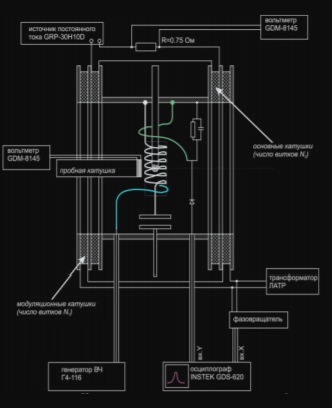
\includegraphics{1.png}
\centering
\caption{Схема установки.}
\end{figure}
Схема установки представлена на Рис. 1. Образец (порошок ДФПГ) в стеклянной ампуле помещается внутрь катушки индуктивности, входящей в состав колебательного контура. Входящий в состав контура конденсатор состоит из двух пластин, разделённых воздушным зазором, одна из пластин может перемещаться поворотом штока. Колебания в контуре возбуждаются антенной, соединённой с генератором высокой частоты (ВЧ) Г4-116. Амплитуда колебаний поля в катушке индуктивности
измеряется по наводимой в петле связи ЭДС индукции. Высокочастотные колебания ЭДС
индукции в приёмном контуре детектируются диодом, измеряемая при помощи
осциллографа низкочастотная огибающая этого сигнала пропорциональна квадрату
амплитуды колебаний поля в катушке.\\
Постоянное магнитное поле создаётся пропусканием тока от источника постоянного тока через основные катушки. При этом при помощи вольтметра измеряется падение напряжения на резисторе в цепи основных катушек. Переменное поле небольшой амплитуды создаётся подачей на модуляционные катушки напряжения с регулируемого трансформатора ЛАТР. Для измерения амплитуды колебаний переменного поля используется пробная катушка известной геометрии, подключённая к вольтметру. Пусть поток через неё $\Phi_{\text{проб}}$, тогда ЭДС индукции
\[\mathcal{E} = - \dfrac{d\Phi_{\text{проб}}}{dt}.\]
Если $I_{\text{осн}}$ — ток через основную катушку, а $M$ — взаимная индуктивность основной и пробной катушек, то
\[\Phi_{\text{проб}} = M I_{\text{осн}}.\]
Тогда амплитудное значение ЭДС индукции
\[\mathcal{E}_{\text{амп}} = - \dfrac{dM I_{\text{осн}}}{dt} = M \omega I_{\text{амп}}.\]
Учитывая, что $I_{\text{амп}} = \sqrt{2} I_{\text{действ}}=\frac{V_r}{r}$, где $V_R$, $R$ — напряжение на резисторе с сопротивлением $R$ в цепи основных катушек, а также $\mathcal{E}_{\text{амп}} = \sqrt{2}\mathcal{E}_{\text{ср}}$, получим
\[\mathcal{E}_{\text{ср}} = M \omega \dfrac{V_R}{R} = k V_R.\]
Тогда, зная, что
\[\Phi_{\text{проб}} = B_0 N_{\text{проб}} \dfrac{\pi d_{\text{проб}}^2}{4} = \dfrac{MU_R}{R} = \dfrac{k U}{\omega},\]
где $U$ — напряжение на $R$ в резонансе, получим
\begin{equation}\label{1}
B_0 = \dfrac{4k U}{\pi \omega d^2_{\text{проб}} N_{\text{проб}}}.
\end{equation}
Характеристики катушек: пробная катушка $N_{\text{проб}} = 49$, $d_{\text{проб}} = 14.5\pm 0.1~\text{мм}$, основная катушка $N_{\text{осн}} = 5500$, $d_{\text{осн}} = 0.25\pm 0.01~\text{м}$, модулирующая катушка $N_{\text{мод}} = 1500$, $d_{\text{мод}} = 0.30\pm 0.01~\text{м}$.
\section*{Ход работы и обработка данных}
1) Настроил установку и снял зависимости резонансной частоты и напряжения катушки, каждый раз меняя емкости конденсатора и настраиваясь на новые резонансы
\begin{table}[h]
\begin{tabular}{|c|c|c|c|c|c|c|c|}
\hline
$f$, МГц & 98 & 110 & 121 & 127 & 134 & 145 & 163 \\ \hline
$V_{\text{кат}}$, мВ & 79.82 & 90.31 & 96.24 & 103.35 & 110.05 & 114.24 & 128.43 \\ \hline
\end{tabular}
\centering
\end{table}\\
2) Настроившись на любой резонанс, поднесем катушку и внесем ее внутрь соленоида максимально близко к образцу и снимем зависимость напряжения на катушки по резонансным напряжениям на зонде.
\begin{table}[h]
\begin{tabular}{|c|c|c|c|c|c|c|c|}
$V_{\text{кат}}$, мВ & 79.48 & 90.69 & 96.87 & 103.08 & 110.26 & 114.45 & 128.20 \\ \hline
$V_{\text{зонд}}$, мВ & 9.44 & 10.65 & 11.35 & 11.87 & 12.50 & 13.21 & 14.66 \\ \hline
\end{tabular}
\centering
\end{table}\\
3) Из уравнения: $U = n B_0 S \omega_n$,
$B_{\text{кат}} =
f(V_{\text{кат})}$
Построим график:
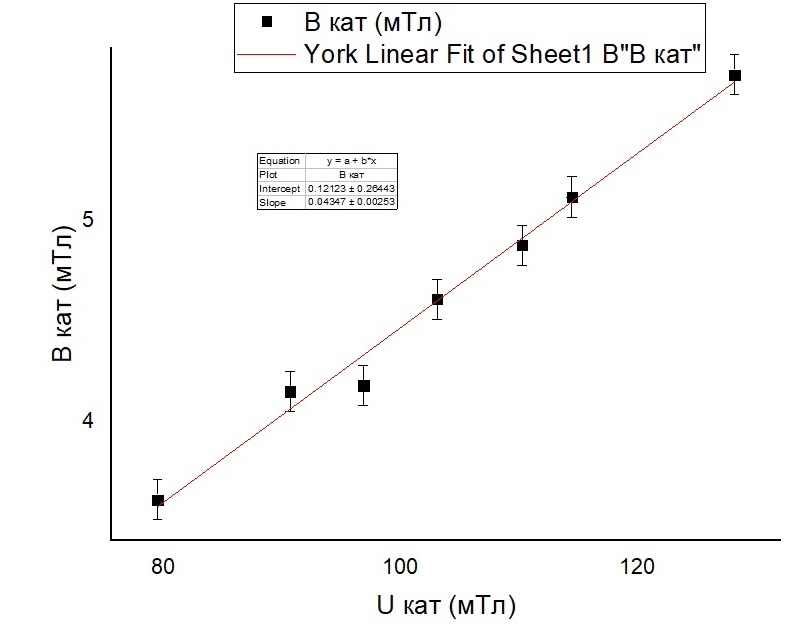
\includegraphics[scale = 0.4]{one.jpg}
\centering

4) Определим g - фактор электрона по формуле: $g = h \omega / \mu B$
\begin{table}[h]
\begin{tabular}{|c|c|c|c|c|c|c|c|}
\hline
$f$, МГц & 98 & 110 & 121 & 127 & 134 & 145 & 163 \\ \hline
$B$, мВ & 3.61 & 4.15 & 4.18 & 4.61 & 4.88 & 5.12 & 5.73 \\ \hline
$g$ & 2.02 & 1.98 & 1.99 & 2.05 & 1.99 & 2.01 & 2.02 \\ \hline
\end{tabular}
\centering
\end{table}\\

Построим график зависимости f от B:
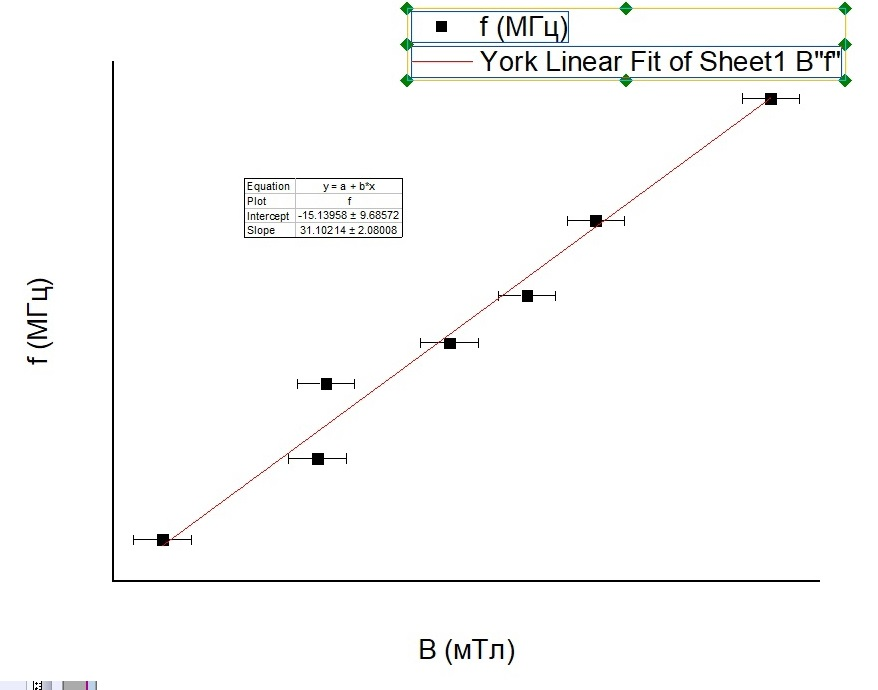
\includegraphics[scale = 0.4]{two.jpg}

5) Посчитаем погрешности:
\[\sigma_g = \sqrt{ \left( \dfrac{\partial g}{\partial f_0}\right)^2 \sigma_{f_0}^2 + \left( \dfrac{\partial g}{\partial B_0}\right)^2 \sigma_{B_0}^2}. = 0.14\]
Итоговое значение g - фактора лежит в пределах погрешности: g = 2.02 +- 0.14

6) Рассчитаем $\Delta B$ через $\Delta V$ по клеткам. Получим $\Delta B = 0.186$. Ширина пика на
половине своей высоты $\Delta B_2 = 0.372$

\section*{Вывод}
В данной работе был исследован ЭПР в молекуле ДФПГ. Определили $g$-фактор электрона $g = 2.02 \pm 0.14$, а также измерена ширина линий ЭПР $\Delta B = 0.186 \pm 0.013~\text{мТл}$. Полученное значение g - фактора попадает с учетом погрешности в табличное (g = 2.0036).
\end{document}